\section{Produktentwicklung}
Die Findung einer passenden Produktidee gestaltete sich unter den im vorherigen Abschnitt erwähnten Bedingungen nicht unbedingt als einfach:

Zwar soll der grösste Teil des Arbeitsaufwandes in das Entwickeln einer beispielhaften Architektur fliessen, diese soll aber in einem für Studierende möglichst attraktiven Gewand präsentiert werden.

Der interessierte Leser findet im Anhang \ref{sec:produktentwicklung} ``\nameref{sec:produktentwicklung}'' weitere Details zum Prozess der konkreten Produktentwicklung. An dieser Stelle soll jedoch der Fokus auf der finalen Idee liegen.


\subsection{Die Produktidee: Roomies}
\emph{Roomies} soll einer \gls{WG} ermöglichen, anfallende Aufgaben leicht unter den verschiedenen Bewohnern zu organisieren. Damit auch langweilige Ämtchen endlich erledigt werden, schafft Roomies durch ein Ranglisten- und Badgesystem (\gls{Gamification}) einen Anreiz, um seine Mitbewohner übertrumpfen zu wollen.

Durch das Aufgreifen einer Thematik aus dem Studentenalltag soll Roomies für Lernende aus dem Modul \emph{Internettechnologien} einen leichten Einstieg in die tendenziell trockene Materie der Softwarearchitektur bieten.

\subsection{Branding}
Der namensgebende Ausdruck \emph{Roomie} stammt aus dem US-amerikanischen und bedeutet soviel wie \emph{Mitbewohner} oder \emph{Zimmernachbar} \cite{Roomie}. Passend dazu soll neben dem Namen auch das restliche Produktbranding an die US-amerikanische College-Welt angelehnt werden.

Vom Logo über die Farbwahl bis zum späteren User Interface Design sollen folgende Stilelemente als roter Faden verwendet werden:

\begin{enumerate}
	\item \emph{Gedimmte} Farben, keine grellen Akzente
	\item Simple, aber eingängige und klar definierte Formensprache
	\item Serifen-betonte Schriftart als Stilmittel
\end{enumerate}

Im Folgenden sind die Grundlegenden Stilelemente zur Referenz aufgeführt. Das Produktlogo wird zudem in verschiedenen, grössenoptimierten Varianten gezeigt.

\subsubsection*{Grundfarbpalette}
\begin{figure}[H]
	\definecolor{spec_white}{HTML}{FFFFFF}
	\definecolor{spec_blue}{HTML}{1A3143}
	\definecolor{spec_red}{HTML}{A4000F}

	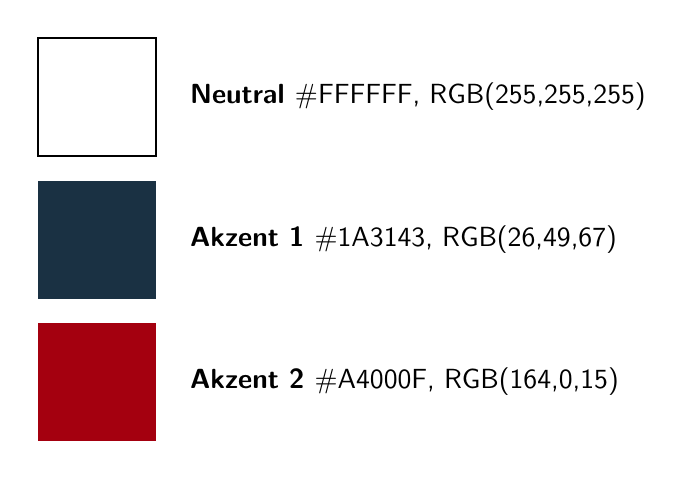
\begin{tikzpicture}
		\tikzstyle{colorswatch} = [rectangle,draw=none,minimum width=15mm,minimum height=15mm,thick];
		\tikzstyle{colorspec} = [draw=none,fill=none,right];

		\matrix[row sep=3mm, column sep=3mm]{
			\node[colorswatch,draw=black,fill=spec_white]{}; &
			\node[colorspec]{\sffamily\bfseries Neutral \normalfont\sffamily\#FFFFFF, RGB(255,255,255)}; \\
			\node[colorswatch,fill=spec_blue]{}; &
			\node[colorspec]{\sffamily\bfseries Akzent 1 \normalfont\sffamily\#1A3143, RGB(26,49,67)}; \\
			\node[colorswatch,fill=spec_red]{}; &
			\node[colorspec]{\sffamily\bfseries Akzent 2 \normalfont\sffamily\#A4000F, RGB(164,0,15)}; \\
		};
	\end{tikzpicture}
	\caption{Branding Farbpalette}
\end{figure}

\subsubsection*{Logo \& Logovariationen}
\begin{figure}[H]
	\centering
	
\includegraphics[width=5cm]{content/images/roomies-withshadow.png}
	\caption{Roomies Logo im College Stil}
\end{figure}

\begin{figure}[H]
	\centering
	
\includegraphics[width=10cm]{content/images/logo-variants.png}
	\caption{Roomies Logo in verschiedenen Grössen \& Varianten}
\end{figure}